\chapter {Interfacing a Servomotor}
\thispagestyle{empty}
\label{sec:servo}
\newcommand{\LocSERfig}{\Origin/user-code/servo/figures}
\newcommand{\LocSERscicode}{\Origin/user-code/servo/scilab}
\newcommand{\LocSERscibrief}[1]{{\tt \seqsplit{%
    Origin/user-code/servo/scilab/#1}},
see \fnrefp{fn:file-loc}}

\newcommand{\LocSERardcode}{\Origin/user-code/servo/arduino}
\newcommand{\LocSERardbrief}[1]{{\tt \seqsplit{%
    Origin/user-code/servo/arduino/#1}}, 
see \fnrefp{fn:file-loc}}

%%%%%%%%%%%%%%%python starts
\newcommand{\LocSERpycode}{\Origin/user-code/servo/python}
\newcommand{\LocSERpybrief}[1]{{\tt \seqsplit{%
    Origin/user-code/servo/python/#1}}, 
see \fnrefp{fn:file-loc}}
%%%%%%%%%%%%%%%python ends

%%%%%%%%%%%%%%%julia starts
\newcommand{\LocSERjuliacode}{\Origin/user-code/servo/julia}
\newcommand{\LocSERjuliabrief}[1]{{\tt \seqsplit{%
    Origin/user-code/servo/julia/#1}}, 
see \fnrefp{fn:file-loc}}
%%%%%%%%%%%%%%%julia ends

%%%%%%%%%%%%%%% OpenModelica starts
\newcommand{\LocSEROpenModelicacode}{\Origin/user-code/servo/OpenModelica}
\newcommand{\LocSEROpenModelicabrief}[1]{{\tt \seqsplit{%
    Origin/user-code/servo/OpenModelica/#1}}, 
see \fnrefp{fn:file-loc}}
%%%%%%%%%%%%%%% OpenModelica ends

A servomotor is a very useful industrial control mechanism.  Learning
to control it will be extremely useful for practitioners.  In this
chapter, we will explain how to control a servomotor using the
\arduino\ board.  We will begin with preliminaries of servomotors and
explain how to connect a typical servomotor to the \arduino\ board and
shield.  We will then explain how to control it through Arduino IDE,
Scilab and Xcos.  We will give code for all the experiments.

\section{Preliminaries}
A servomotor is a rotary control mechanism.  It can be commanded to
rotate to a specified angle.  It can rotate in positive or negative
direction.  Using servomotors, one can control
angular position, velocity and acceleration.  Servomotors are useful
in many applications.  Some examples are robotics, industrial motors
and printers.

Typical servomotors have a maximum range of $180^\circ$, although some
have different ranges\footnote{All the angles in a servomotor are
  absolute angles, with respect to a fixed reference point, which can
  be taken as $0^\circ$.}
Servomotors typically have a position sensor,
using which, rotate to the commanded angle.  The minimum angle to
which a servomotor can be rotated is its least count, which varies
from one model to another.  Low cost servomotors have a large least
count, say, of the order of $10^\circ$.

A servomotor typically comes with three terminals for the
following three signals: position signal (PWM), Vcc and ground.
We now explain how to connect a typical servomotor to the \arduino\
board, through \tabref{tab:servo-connect}.
\begin{table}
\centering
\caption{Connecting a typical servomotor to \arduino\ board}
\label{tab:servo-connect}
\begin{tabular}{lc}\hline
Servomotor terminal & Arduino board \\ \hline
Position signal & 9 \\
Ground (black/brown wire) & Ground \\ 
Vcc (red or orange middle-wire) & 5V \\
Signal (orange or yellow) & Pin 9 \\ \hline
\end{tabular}
\end{table}

\section{Controlling the Servometer through the Arduino IDE}
\subsection{Controlling the Servometer}
\label{sec:servo-ard}
In this section, we will describe some experiments that will help
rotate the servomotor based on the command given from Arduino IDE.  We
will also give the necessary code.  We will present four experiments
in this section.  The shield has to be attached to the \arduino\ board
before doing these experiments.  The reader should go through the
instructions given in \secref{sec:ard-start} before getting started.
\begin{enumerate}
%\setcounter{enumi}{-1}
\item In the first experiment, we will move the servomotor by
  $30^\circ$ using \ardref{ard:servo-init}.  Line 1 of this code
  includes a header file that initializes some of the parameters.
  Line 2 creates a {\tt Servo} object and calls it {\tt myservo}.
  Most Arduino boards allow the creation of 12 servo objects.  Line 4
  commands myservo to be attached to pin 9.  Line 5 asks the
  servomotor to rotate by $90^\circ$.  Other commands are as in the
  previous chapters.

  Once this code is executed, the servomotor would move by
  $30^\circ$, as commanded.  What happens if this code is executed
  once again?  The motor will not move at all.  What is the reason?
  Recall that what we assign to the motor are absolute positions, with
  respect to a fixed origin.  As a result, there will be no change at
  all. 

\item In the second experiment, we move the motor by $90^\circ$ in the
  forward direction and $45^\circ$ in the reverse direction.  This
  code is given in \ardref{ard:servo-reverse}.  In Line 6, we provide
  a delay of one second.  What is the reason?  If the delay were not
  there, the motor will move only by the net angle of $90-45 = 45$
  degrees.  The reader should verify this by commenting on the delay
  command.

\item In the third experiment, we move the motor in increments of
  $20^\circ$.  This is achieved by the for loop, as in
  \ardref{ard:servo-loop}.  Both {\tt i}, the loop variable and {\tt
    angle}, the variable to store angle, are declared as {\tt int} in
  this code.  The code helps the motor move in steps of $20^\circ$ all
  the way to $180^\circ$.  Please see below a few exercise questions.

\item Finally, in the last experiment, we read the potentiometer value
  from the shield and use it to drive the servomotor, see
  \ardref{ard:servo-pot}.  The resistance of the potentiometer is
  represented in 10 bits.  As a result, the resistance value could be
  any one of 1,024 values, from 0 to 1,023.  This entire range is
  mapped to $180^\circ$.  By rotating the potentiometer, one can make
  the motor move by different amounts.

  The potentiometer is connected to pin number 2.  Through this pin,
  the resistance of the potentiometer, in the range of 0 to 1,023,
  depending on its position, is read.  Thus, by rotating the
  potentiometer, we make different values appear on pin 2.  This value
  is used to move the servo.  For example, if the resistance is half
  of the total, the servomotor will go to $90^\circ$ and so on.  The
  servomotor stops for half a second after every move.  The loop is
  executed 5,000 times, with half a second delay for each iteration.
  During this period, the servomotor keeps moving as dictated by the
  resistance of the potentiometer.

\end{enumerate}

\begin{exercise}
Let us carry out this exercise:
\begin{enumerate}
\item In \ardref{ard:servo-loop}, the loop parameter {\tt i} starts
  from 1.  From what angle will the motor start?  If one wants the
  motor to start from $0^\circ$, what should one do?
\item How does one find the least count of the servomotor?  If the
  variable {\tt angle} is chosen to be less than this least count in
  \ardref{ard:servo-loop}, what happens?
\item What happens if 180 in Line 10 of \ardref{ard:servo-pot} is
  changed to 90?  What does the change 180 to 90 mean?
\end{enumerate}
\end{exercise}

\subsection{Arduino Code}
\lstset{style=mystyle}
\label{sec:servo-arduino-code}
\addtocontents{ard}{\protect\addvspace{\codclr}}

\begin{ardcode}
  \acaption{Rotating the servomotor to a specified degree} {Rotating
    the servomotor to a specified degree.  Available at
    \LocSERardbrief{servo-init/servo-init.ino}.}
  \label{ard:servo-init}
  \lstinputlisting{\LocSERardcode/servo-init/servo-init.ino}
\end{ardcode}

\begin{ardcode}
  \acaption{Rotating the servomotor to a specified degree and
    reversing} {Rotating 
    the servomotor to a specified degree and reversing.  Available at
    \LocSERardbrief{servo-reverse/servo-reverse.ino}.}
  \label{ard:servo-reverse}
  \lstinputlisting{\LocSERardcode/servo-reverse/servo-reverse.ino}
\end{ardcode}

\begin{ardcode}
  \acaption{Rotating the servomotor in increments} {Rotating the
    servomotor in increments.  Available at
    \LocSERardbrief{servo-loop/servo-loop.ino}.}
  \label{ard:servo-loop}
  \lstinputlisting{\LocSERardcode/servo-loop/servo-loop.ino}
\end{ardcode}

\begin{ardcode}
  \acaption{Rotating the servomotor through the potentiometer}
  {Rotating the servomotor through the potentiometer.  Available at
    \LocSERardbrief{servo-pot/servo-pot.ino}.}
  \label{ard:servo-pot}
  \lstinputlisting{\LocSERardcode/servo-pot/servo-pot.ino}
\end{ardcode}

\section{Controlling the Servomotor through Scilab}
\subsection{Controlling the Servomotor}
\label{sec:servo-sci}
In this section, we will carry out the servomotor control experiments
using \scilab.  We will follow the same order as in
\secref{sec:servo-ard}.  We assume that the shield is attached to the
\arduino\ board while doing these experiments.  They will work without
the shield also, but in this case, our comments on colour LEDs
lighting will not be applicable.  The reader should go through the
instructions given in \secref{sec:sci-start} before getting started.
\begin{enumerate}
\item The first experiment makes the servomotor move by $30^\circ$,
  the code for which is given in \ardref{sci:servo-init}.
  It first opens com port 2 in \arduino\ card number 1 with baud rate
  of 115200.  If the port opening is unsuccessful {\tt ok} will not be
  0 and the program terminates, asking the user to correct the
  problem.  Else If the port opening is successful, {\tt ok} will be 0
  and the program proceeds.  In Line number 3 of the code, \ie\
  \lstinputlisting[firstline=3,lastline=3]{\LocSERscicode/servo-init.sce}
  we say that the servomotor is attached on board 1 (the first entry)
  to pin 1 (the second entry).  In the \scilab\ toolbox, pin 1 and pin
  9 are connected and as a result, we connect the wire physically to
  pin 9.  Similarly, pins 2 and 10 are connected through the
  \scilab\ toolbox.

\item In \sciref{sci:servo-reverse}, we make the servomotor rotate
  to $90^\circ$, wait for a second and go to $45^\circ$.  As mentioned
  earlier, the angles are absolute with respect to a fixed reference
  point and not relative.  

\item In the next experiment, we rotate the servomotor in discrete
  steps of $20^\circ$.  This is achieved by multiplying $20^\circ$ by
  an integer {\tt i}, which varies from 0 to 10.  Once the maximum
  angle reaches $180^\circ$, it stops.  

\item Finally, in the last experiment, we position the servomotor
  through the potentiometer in the code \sciref{sci:servo-pot}.  As we
  rotate the potentiometer, the servomotor's angle also changes.  The
  potentiometer value is read through pin 2, in line number 5, as
  below:
  \lstinputlisting[firstline=5,lastline=5]{\LocSERscicode/servo-pot.sce}
  This value is mapped into a value between 0 and $180^\circ$ by
  multiplying with $180/1023$ in line 6:
  \lstinputlisting[firstline=6,lastline=6]{\LocSERscicode/servo-pot.sce}
  The {\tt floor} function gets the integer part of the number by
  truncation.  This is the angle by which the potentiometer is to be
  moved.  Truncation is a not a crucial calculation, however.  In
  every iteration, the servomotor's position is calculated, and placed
  for half a second.  This loop is iterated upon 5,000 times.
\end{enumerate}

\subsection{Scilab Code}
\lstset{style=mystyle}
\label{sec:servo-scilab-code}
\addtocontents{cod}{\protect\addvspace{\codclr}}

\begin{scicode}
  \ccaption{Rotating the servomotor to a specified degree} {Rotating
    the servomotor to a specified degree.  Available at
    \LocSERscibrief{servo-init.sce}.}
  \label{sci:servo-init}
  \lstinputlisting{\LocSERscicode/servo-init.sce}
\end{scicode}

\begin{scicode}
  \ccaption{Rotating the servomotor to a specified degree and
    reversing} {Rotating 
    the servomotor to a specified degree and reversing.  Available at
    \LocSERscibrief{servo-reverse.sce}.}
  \label{sci:servo-reverse}
  \lstinputlisting{\LocSERscicode/servo-reverse.sce}
\end{scicode}

\begin{scicode}
  \ccaption{Rotating the servomotor in steps of $20^\circ$}{Rotating
    the servomotor in steps of $20^\circ$.  Available at 
    \LocSERscibrief{servo-loop.sce}.}
  \label{sci:servo-loop}
  \lstinputlisting{\LocSERscicode/servo-loop.sce}
\end{scicode}

\begin{scicode}
  \ccaption{Rotating the servomotor to a degree specified by the
    potentiometer} {Rotating the servomotor to a degree specified by
    the potentiometer.  Available at \LocSERscibrief{servo-pot.sce}.}
  \label{sci:servo-pot}
  \lstinputlisting{\LocSERscicode/servo-pot.sce}
\end{scicode}


\section{Controling the Servomotor through Xcos}
\label{sec:servo-xcos}
In this section, we will see how to rotate the servomotor from Scilab
Xcos.  We will carry out experiments similar to the ones in earlier
sections.  For each, we will give the location of the zcos file and
the parameters to set.  The reader should go through the instructions
given in \secref{sec:xcos-start} before getting started.

\begin{enumerate}
\item First we will rotate the servomotor by $30^\circ$.  When
  the file required for this experiment is invoked, one gets the GUI
  as in \figref{fig:servo-init}.  In the caption of this figure, one can
  see where to locate the file.
  \begin{figure}
    \centering
    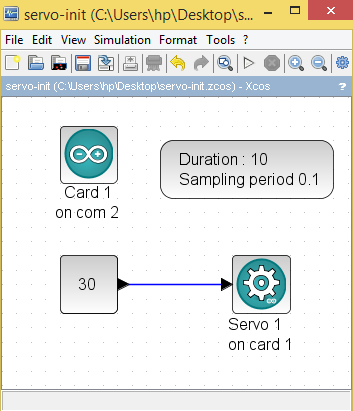
\includegraphics[width=\smfig]{\LocSERfig/servo-init.png}
    \caption[Rotating the servomotor by a fixed angle]{Rotating the
    servomotor by a fixed angle.  This is what one sees when
        \LocLEDscibrief{servo-init.zcos}, is invoked.}
    \label{fig:servo-init}
  \end{figure}

  We will next explain how to set the parameters for this simulation.
  To set value on any block, one needs to right click and open the
  {\tt Block Parameters} or double click.  The values for each block
  is tabulated in \tabref{tab:servo-init}.  All other parameters are to
  be left unchanged.
  \begin{table}
    \centering
    \caption{Parameters to rotate the servomotor by $30^\circ$}
    \label{tab:servo-init}
    \begin{tabular}{llc} \hline
      Name of the block & Parameter name & Value \\ \hline
      ARDUINO\_SETUP & Identifier of Arduino Card & 1 \\
      & Serial com port number & 2\portcmd \\ \hline
      TIME\_SAMPLE & Duration of acquisition(s) & 10 \\
      & Sampling period(s) & 0.1 \\ \hline
      SERVO\_WRITE\_SB & Servo number & 1 \\
      & Arduino card number & 1 \\ \hline
      CONST\_m & Constant value & 30 \\ \hline
    \end{tabular}
  \end{table}

\item Next, we will rotate the servomotor by $90^\circ$ and bring it
  to $45^\circ$, all absolute values.  When the file required for this
  experiment is invoked, one gets the GUI as in
  \figref{fig:servo-reverse}.  In the caption of this figure, one can
  see where to locate the file.
  \begin{figure}
    \centering
    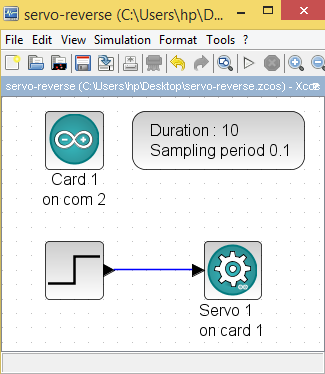
\includegraphics[width=\smfig]{\LocSERfig/servo-reverse.png}
    \caption[Rotating the servomotor forward and then
    reverse]{Rotating the servomotor forward and then reverse.  This
      is what one sees when \LocLEDscibrief{servo-reverse.zcos},
      is invoked.}
    \label{fig:servo-reverse}
  \end{figure}

  We will next explain how to set the parameters for this simulation.
  To set value on any block, one needs to right click and open the
  {\tt Block Parameters} or double click.  The values for each block
  is tabulated in \tabref{tab:servo-reverse}.  All other parameters
  are to be left unchanged.
  \begin{table}
    \centering
    \caption{Parameters to rotate the servomotor forward and reverse}
    \label{tab:servo-reverse}
    \begin{tabular}{llc} \hline
      Name of the block & Parameter name & Value \\ \hline
      ARDUINO\_SETUP & Identifier of Arduino Card & 1 \\
      & Serial com port number & 2\portcmd \\ \hline
      TIME\_SAMPLE & Duration of acquisition(s) & 10 \\
      & Sampling period(s) & 0.1 \\ \hline
      SERVO\_WRITE\_SB & Servo number & 1 \\
      & Arduino card number & 1 \\ \hline
      STEP\_FUNCTION & Step time & 1 \\ 
      & Initial value & 90 \\
      & Final value & 45 \\ \hline
    \end{tabular}
  \end{table}

\item Next, we will rotate the servomotor in increments of
  $20^\circ$.  When the file required for this
  experiment is invoked, one gets the GUI as in
  \figref{fig:servo-loop}.  In the caption of this figure, one can
  see where to locate the file.
  \begin{figure}
    \centering
    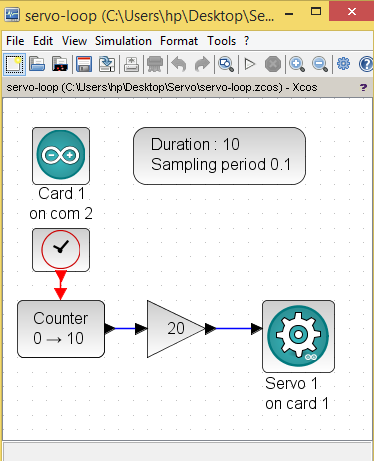
\includegraphics[width=\smfig]{\LocSERfig/servo-loop.png}
    \caption[Rotating the servomotor in increments of $20^\circ$]
    {Rotating the servomotor in increments of $20^\circ$.  This is what
      one sees when \LocLEDscibrief{servo-loop.zcos}, is invoked.}
    \label{fig:servo-loop}
  \end{figure}

  We will next explain how to set the parameters for this simulation.
  To set value on any block, one needs to right click and open the
  {\tt Block Parameters} or double click.  The values for each block
  is tabulated in \tabref{tab:servo-loop}.  {\tt Do on Overflow 0}
  means that we need to do nothing when there is an overflow.
  All other parameters
  are to be left unchanged.
  \begin{table}
    \centering
    \caption{Parameters to make the servomotor to sweep the entire
      range in increments}
    \label{tab:servo-loop}
    \begin{tabular}{llc} \hline
      Name of the block & Parameter name & Value \\ \hline
      ARDUINO\_SETUP & Identifier of Arduino Card & 1 \\
      & Serial com port number & 2\portcmd \\ \hline
      TIME\_SAMPLE & Duration of acquisition(s) & 10 \\
      & Sampling period(s) & 0.1 \\ \hline
      SERVO\_WRITE\_SB & Servo number & 1 \\ \hline
      CLOCK\_c & Period & 1 \\
      & Initialization time & 0.1 \\ \hline
      Counter & Minimum value & 0 \\
      & Maximum value & 10 \\ 
      & Rule & 1 \\ \hline
      GAINBLK & Gain & 20 \\
      & Do on overflow & 0 \\ \hline
    \end{tabular}
  \end{table}

\item Finally, we will use Xcos to rotate the servomotor as per the
  input received from the potentiometer.  When the file required for
  this experiment is invoked, one gets the GUI as in
  \figref{fig:servo-pot}.  In the caption of this figure, one can see
  where to locate the file.
  \begin{figure}
    \centering
    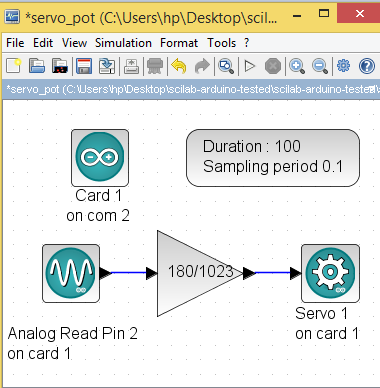
\includegraphics[width=\smfig]{\LocSERfig/servo-pot.png}
    \caption[Rotating the servomotor as suggested by the
    potentiometer]{Rotating the servomotor as suggested by the
    potentiometer.  This is what
      one sees when \LocLEDscibrief{servo-pot.zcos}, is invoked.}
    \label{fig:servo-pot}
  \end{figure}

  We will next explain how to set the parameters for this simulation.
  To set value on any block, one needs to right click and open the
  {\tt Block Parameters} or double click.  The values for each block
  is tabulated in \tabref{tab:servo-pot}.  All other parameters are to
  be left unchanged.  The {\tt ANALOG\_READ\_SB} block reads the value
  of potentiometer and is converted into rotation angle (180/1023),
  computed by {\tt GAIN\_f}.
  \begin{table}
    \centering
    \caption{Parameters to rotate the servomotor based on the input
      from the potentiometer}
    \label{tab:servo-pot}
    \begin{tabular}{llc} \hline
      Name of the block & Parameter name & Value \\ \hline
      ARDUINO\_SETUP & Identifier of Arduino Card & 1 \\
      & Serial com port number & 2\portcmd \\ \hline
      TIME\_SAMPLE & The duration of acquisition(s) & 100 \\
      & Sampling period(s) & 0.1 \\ \hline
      SERVO\_WRITE\_SB & Servo number & 1 \\ \hline
      ANALOG\_READ\_SB & Analog Pin & 2 \\ 
      & Arduino card number & 1 \\ \hline
      GAIN\_f & Gain & 180/1023 \\ \hline
    \end{tabular}
  \end{table}
\end{enumerate}


\section{Controlling the Servomotor through Python}
\subsection{Controlling the Servomotor}
\label{sec:servo-py}
In this section, we will carry out the servomotor control experiments
using python.  We will follow the same order as in
\secref{sec:servo-ard}.  We assume that the shield is attached to the
\arduino\ board while doing these experiments.  They will work without
the shield also, but in this case, our comments on colour LEDs
lighting will not be applicable.  The reader should go through the
instructions given in \secref{sec:py-start} before getting started.
\begin{enumerate}
\item The first experiment makes the servomotor move by $30^\circ$,
  the code for which is given in \ardref{py:servo-init}.
  It first opens com port 2 in \arduino\ card number 1 with baud rate
  of 115200.  If the port opening is unsuccessful {\tt ok} will not be
  0 and the program terminates, asking the user to correct the
  problem.  Else If the port opening is successful, {\tt ok} will be 0
  and the program proceeds.  In Line number 3 of the code, \ie\
  \lstinputlisting[firstline=3,lastline=3]{\LocSERpycode/servo-init.py}
  we say that the servomotor is attached on board 1 (the first entry)
  to pin 1 (the second entry).  In the \scilab\ toolbox, pin 1 and pin
  9 are connected and as a result, we connect the wire physically to
  pin 9.  Similarly, pins 2 and 10 are connected through the
  \scilab\ toolbox.

\item In \sciref{py:servo-reverse}, we make the servomotor rotate
  to $90^\circ$, wait for a second and go to $45^\circ$.  As mentioned
  earlier, the angles are absolute with respect to a fixed reference
  point and not relative.  

\item In the next experiment, we rotate the servomotor in discrete
  steps of $20^\circ$.  This is achieved by multiplying $20^\circ$ by
  an integer {\tt i}, which varies from 0 to 10.  Once the maximum
  angle reaches $180^\circ$, it stops.  

\item Finally, in the last experiment, we position the servomotor
  through the potentiometer in the code \pyref{py:servo-pot}.  As we
  rotate the potentiometer, the servomotor's angle also changes.  The
  potentiometer value is read through pin 2, in line number 5, as
  below:
  \lstinputlisting[firstline=5,lastline=5]{\LocSERpycode/servo-pot.py}
  This value is mapped into a value between 0 and $180^\circ$ by
  multiplying with $180/1023$ in line 6:
  \lstinputlisting[firstline=6,lastline=6]{\LocSERpycode/servo-pot.py}
  The {\tt floor} function gets the integer part of the number by
  truncation.  This is the angle by which the potentiometer is to be
  moved.  Truncation is a not a crucial calculation, however.  In
  every iteration, the servomotor's position is calculated, and placed
  for half a second.  This loop is iterated upon 5,000 times.
\end{enumerate}

\subsection{Python Code}
\lstset{style=mystyle}
\label{sec:servo-python-code}
\addtocontents{pyd}{\protect\addvspace{\codclr}}

\begin{pycode}
  \pcaption{Rotating the servomotor to a specified degree} {Rotating
    the servomotor to a specified degree.  Available at
    \LocSERpybrief{servo-init.py}.}
  \label{py:servo-init}
  \lstinputlisting{\LocSERpycode/servo-init.py}
\end{pycode}

\begin{pycode}
  \pcaption{Rotating the servomotor to a specified degree and
    reversing} {Rotating 
    the servomotor to a specified degree and reversing.  Available at
    \LocSERpybrief{servo-reverse.py}.}
  \label{py:servo-reverse}
  \lstinputlisting{\LocSERpycode/servo-reverse.py}
\end{pycode}

\begin{pycode}
  \pcaption{Rotating the servomotor in steps of $20^\circ$}{Rotating
    the servomotor in steps of $20^\circ$.  Available at 
    \LocSERpybrief{servo-loop.py}.}
  \label{sci:servo-loop}
  \lstinputlisting{\LocSERpycode/servo-loop.py}
\end{pycode}

\begin{pycode}
  \pcaption{Rotating the servomotor to a degree specified by the
    potentiometer} {Rotating the servomotor to a degree specified by
    the potentiometer.  Available at \LocSERpybrief{servo-pot.py}.}
  \label{py:servo-pot}
  \lstinputlisting{\LocSERpycode/servo-pot.py}
\end{pycode}

\section{Controlling the Servomotor through Julia}
\subsection{Controlling the Servomotor}
\label{sec:servo-julia}
In this section, we will carry out the servomotor control experiments
using julia.  We will follow the same order as in
\secref{sec:servo-ard}.Initial cheking of the setup will be same as
described in python.

\begin{enumerate}
\item The first experiment makes the servomotor move by $30^\circ$,
  the code for which is given in \ardref{julia:servo-init}.
  It first opens com port 2 in \arduino\ card number 1 with baud rate
  of 115200.  In Line number 3 of the code, \ie\
  \lstinputlisting[firstline=5,lastline=5]{\LocSERjuliacode/servo-init.jl}
  we say that the servomotor is attached to pin 1 of the board.
  In the julia toolbox, pin 1 and pin
  9 are connected and as a result, we connect the wire physically to
  pin 9.  Similarly, pins 2 and 10 are connected through the
  julia toolbox.

\item In \sciref{julia:servo-reverse}, we make the servomotor rotate
  to $90^\circ$, wait for a second and go to $45^\circ$.  As mentioned
  earlier, the angles are absolute with respect to a fixed reference
  point and not relative.  

\item In the next experiment, we rotate the servomotor in discrete
  steps of $20^\circ$.  This is achieved by multiplying $20^\circ$ by
  an integer {\tt i}, which varies from 0 to 10.  Once the maximum
  angle reaches $180^\circ$, it stops.  

\item Finally, in the last experiment, we position the servomotor
  through the potentiometer in the code \juliaref{julia:servo-pot}.  As we
  rotate the potentiometer, the servomotor's angle also changes.  The
  potentiometer value is read through pin 2, in line number 7, as
  below:
  \lstinputlisting[firstline=7,lastline=7]{\LocSERjuliacode/servo-pot.jl}
  This value is mapped into a value between 0 and $180^\circ$ by
  multiplying with $180/1023$ in line 8:
  \lstinputlisting[firstline=8,lastline=8]{\LocSERjuliacode/servo-pot.jl}
  The {\tt floor} function gets the integer part of the number by
  truncation.  This is the angle by which the potentiometer is to be
  moved.  Truncation is a not a crucial calculation, however.  In
  every iteration, the servomotor's position is calculated, and placed
  for half a second.  This loop is iterated upon 500 times.
\end{enumerate}

\subsection{Julia Code}
\lstset{style=mystyle}
\label{sec:servo-julia-code}
\addtocontents{juliad}{\protect\addvspace{\codclr}}

\begin{juliacode}
  \jcaption{Rotating the servomotor to a specified degree} {Rotating
    the servomotor to a specified degree.  Available at
    \LocSERjuliabrief{servo-init.jl}.}
  \label{julia:servo-init}
  \lstinputlisting{\LocSERjuliacode/servo-init.jl}
\end{juliacode}

\begin{juliacode}
  \jcaption{Rotating the servomotor to a specified degree and
    reversing} {Rotating 
    the servomotor to a specified degree and reversing.  Available at
    \LocSERjuliabrief{servo-reverse.jl}.}
  \label{julia:servo-reverse}
  \lstinputlisting{\LocSERjuliacode/servo-reverse.jl}
\end{juliacode}

\begin{juliacode}
  \jcaption{Rotating the servomotor in steps of $20^\circ$}{Rotating
    the servomotor in steps of $20^\circ$.  Available at 
    \LocSERjuliabrief{servo-loop.jl}.}
  \label{julia:servo-loop}
  \lstinputlisting{\LocSERjuliacode/servo-loop.jl}
\end{juliacode}

\begin{juliacode}
  \jcaption{Rotating the servomotor to a degree specified by the
    potentiometer} {Rotating the servomotor to a degree specified by
    the potentiometer.  Available at \LocSERjuliabrief{servo-pot.jl}.}
  \label{julia:servo-pot}
  \lstinputlisting{\LocSERjuliacode/servo-pot.jl}
\end{juliacode}

\section{Controlling the Servomotor through OpenModelica}
\subsection{Controlling the Servomotor}
\label{sec:servo-OpenModelica}
In this section, we will carry out the servomotor control experiments
using OpenModelica.  We will follow the same order as in
\secref{sec:servo-ard}.Initial cheking of the setup will be same as
described in python.

\begin{enumerate}
\item The first experiment makes the servomotor move by $30^\circ$,
  the code for which is given in \OpenModelicaref{OpenModelica:servo-init}.
  It first opens com port 0 in \arduino\ card number 1 with baud rate
  of 115200.  In Line number 09 of the code, \ie\
  \lstinputlisting[firstline=9,lastline=9]{\LocSEROpenModelicacode/servo-init.mo}
  we say that the servomotor is attached to pin 1 of the board.
  As previously explained, pin 1 and pin 9 are also connected in OpenModelica
  toolbox.

\item In \OpenModelicaref{OpenModelica:servo-reverse}, we make the servomotor rotate
  to $90^\circ$, wait for a second and go to $45^\circ$.  As mentioned
  earlier, the angles are absolute with respect to a fixed reference
  point and not relative.  

\item In the next experiment, we rotate the servomotor in discrete
  steps of $20^\circ$.  This is achieved by multiplying $20^\circ$ by
  an integer {\tt i}, which varies from 0 to 10.  Once the maximum
  angle reaches $180^\circ$, it stops.  

\item Finally, in the last experiment, we position the servomotor
  through the potentiometer in the code \OpenModelicaref{OpenModelica:servo-pot}.  As we
  rotate the potentiometer, the servomotor's angle also changes.  The
  potentiometer value is read through pin 2, in line number 7, as
  below:
  \lstinputlisting[firstline=18,lastline=18]{\LocSEROpenModelicacode/servo_pot.mo}
  This value is mapped into a value between 0 and $180^\circ$ by
  multiplying with $180/1023$ in line 8:
  \lstinputlisting[firstline=19,lastline=19]{\LocSEROpenModelicacode/servo_pot.mo}
  The {\tt floor} function gets the integer part of the number by
  truncation.  This is the angle by which the potentiometer is to be
  moved.  Truncation is a not a crucial calculation, however.  In
  every iteration, the servomotor's position is calculated, and placed
  for half a second.  This loop is iterated upon 500 times.

  \end{enumerate}

\subsection{OpenModelica Code}
\lstset{style=mystyle}
\label{sec:servo-OpenModelica-code}
\addtocontents{OpenModelicad}{\protect\addvspace{\codclr}}

\begin{OpenModelicacode}
  \mcaption{Rotating the servomotor to a specified degree} {Rotating
    the servomotor to a specified degree.  Available at
    \LocSEROpenModelicabrief{servo-init.mo}.}
  \label{OpenModelica:servo-init}
  \lstinputlisting{\LocSEROpenModelicacode/servo-init.mo}
\end{OpenModelicacode}

\begin{OpenModelicacode}
  \mcaption{Rotating the servomotor to a specified degree and
    reversing} {Rotating 
    the servomotor to a specified degree and reversing.  Available at
    \LocSEROpenModelicabrief{servo-reverse.mo}.}
  \label{OpenModelica:servo-reverse}
  \lstinputlisting{\LocSEROpenModelicacode/servo-reverse.mo}
\end{OpenModelicacode}

\begin{OpenModelicacode}
  \mcaption{Rotating the servomotor in steps of $20^\circ$}{Rotating
    the servomotor in steps of $20^\circ$.  Available at 
    \LocSERjuliabrief{servo-loop.mo}.}
  \label{OpenModelica:servo-loop}
  \lstinputlisting{\LocSEROpenModelicacode/servo-loop.mo}
\end{OpenModelicacode}

\begin{OpenModelicacode}
  \mcaption{Rotating the servomotor to a degree specified by the
    potentiometer} {Rotating the servomotor to a degree specified by
    the potentiometer.  Available at \LocSEROpenModelicabrief{servo\_pot.mo}.}
  \label{OpenModelica:servo-pot}
  \lstinputlisting{\LocSEROpenModelicacode/servo_pot.mo}
\end{OpenModelicacode}
